%!TEX root = ../thesis.tex

\chapter{Approach}
\label{ch:approach}

In this chapter we discuss how this project was approached.

Though the project itself is fairly straight forward, how to approach it became quite challenging.
Planning out how to implement the desired features in a good and approachable manner, would prove highly time consuming and hard.
Even the desired features themselves were hard enough to conceptualise.
A problem that was not helped by the fact that there was no clear single source of information to describe them.
As a consequence, the approach to this project was always changing, as new desires and ideas were discussed.

In this chapter we discuss this ever changing approach.
How it started as a continuation of previous approaches and a desired workflow.
And how it eventually was altered to combat the rising challenges and issues that were faced.
 
\section{Existing Approach}

The existing approach to this project is detailed in the report written by Adil.

In short, his approach is summarized as follows.
When a teacher creates an assignment, they have the option of creating any number of task markdown files.
For each of these markdown files, a single issue should be created on every student repository.
The title and body of these issues are defined by the contents of the corresponding task.
When a student wants to complete a task, they create a pull request for the associated issue.
After the deadline of the assignment has passed, QuickFeed randomly assigns co-student and teacher reviewers to the pull request. 
Only when the pull request has been approved by a teacher, should it be merged.

Adil discusses several challenges to this approach, and gives his proposed solutions.
Given that he did not finish his work however, many of these solutions have later proved inadequate or faulty, and in some cases, far too complex.
In general, this thesis is independent of the aforementioned approach, and uses it primarily as a source of inspiration.

\section{Desired workflow}

This section describes in detail the desired student and teacher workflow, and is in essence what we want to achieve with this project.

Tasks will be handled as described in the previous section.
They are created by the teacher as markdown files within an assignment, and QuickFeed creates issues based on them.
When a student wants to complete any task, they create a new branch on their local repository.
Using this branch, they create a pull request on their student repository that is linked to the associated issue.

At this stage, a student has an open pull request on their repository.
Tests are run on the student code by QuickFeed, and students receive feedback on these tests via GitHub workflows.

When students are finished with a task, i.e., they receive a passing score from the test results, their code is ready to be reviewed.
At this point, QuickFeed should automatically assign reviewers who should request any changes they deem fitting.
One of these reviewers should always be a teacher.
When all changes are implemented, the teacher approves the pull request, allowing the student to merge it.
Finally, when all tasks have gone through this process, the assignment itself can be set as approved.

We generally approach this project with a desire to make QuickFeed support this workflow.

\section{Challenges}

In the previous section we looked at what exactly it is we are trying to accomplish. 
A number of challenges become apparent when trying to implement these new features however.
In this section we discuss these challenges, as well as how to possibly overcome them.

\subsection{Increased Complexity}

Introducing pull requests to students can prove challenging in itself.
Even though pull requests are not exactly a challenging feature to learn and use, it can still prove time consuming for certain students.
Even more so if students are already struggling with how to use git.
Having to swap between branches, making commits to them, and also knowing how to manage and create pull requests, are all things students will have to familiar with.
More time and effort from the teaching staff may therefore have to be dedicated to assisting students with issues they may have.

This is not an issue that can be explicitly solved.
Every teacher will have to decide themselves if the benefits outweigh the increased complexity when using tasks and pull request with their assignments.

\subsection{Access to Student Repositories}

In order for one student to review the source code of another, they will have to somehow be given access to that code.

A solution could be to use GitHub teams to grant students review access to other repositories.
Access can then be removed once the review process is finished.
This solution does however lead to possible complications.
First of all, students having access to another random student's repository can be somewhat invasive.
Secondly it can lead to the following possible scenario:

Imagine we have two students: Student-1 and Student-2.
Student-2 feels they are finished with a task from assignment1, and therefore requests a review.
Student-1 is assigned to review it, and is granted access by QuickFeed to Student-2's repository.
Student-2 is also diligent, and has already started working on assignment2.
In fact, Student-2 has nearly completed assignment2.
Student-1 however, has not even started on assignment2, but because they can now access Student-2's assignments, they receive valuable knowledge on how to solve it.
Of course, this would be highly problematic to any teacher wanting their students to solve assignments independently.
Any implementation will have to avoid this type of scenario.

Another possible solution is to create a clone repository, containing only the task that is to be reviewed. 
This way, any reviewing student will only have access to the task in question, and not the rest of that students repository.
This solution will therefore avoid the problem described in the above scenario.

A functional implementation of the above solution seems highly complex, as there is a myriad of complications and problems that will have to be accounted for.
For one, if an assignment contains for example 6 tasks, it would mean that 6 copy repositories will have to be created and managed by QuickFeed for each student.
If a course has 50 enrolled students, 300 new repositories will then have to be created, for just that one assignment.
Obviously this is not a feasible way to tackle this issue.

Even if we manage to reduce the number of such repositories that need to be created, there is still the problem of how to manage them.
An implementation needs to handle, amongst other things, the following:

\begin{itemize}
    \item How to create new review repositories containing only the code that is relevant.
    \item How to delete them when they are no longer needed.
    \item How to associate actions between a review repository and the original student repository.
          E.g. if code is updated in the original, should it then also be updated in the other?
          And if so, how do we accomplish this?
    \item How to fit pull requests into this approach.
\end{itemize}

Let us say that we, despite these challenges, managed to create a fully functional implementation of the above solution.
We now have to cope with the prospect that we have further complexified the user experience.
Students having to learn GitHub pull requests may be problematic enough on its own, but also introducing them to review repositories could prove counter-productive.

\subsection{Assigning reviewers}

One of the primary reasons for using GitHub pull requests is to use its code review features.
We want both students and teachers to review code, with teachers explicitly having to approve a pull request for the assignment as a whole to be approved.

When assigning students we must make sure that no student is assigned to review a task they themselves have not yet completed.
Otherwise, we get a similar situation to the one mentioned in the previous challenge, where students have the option of plagiarising other students code.
Any implementation will have to make sure that students reviewing code, should only review code they are themselves already finished with.
A natural approach to this could be to have students only review code when the assignment deadline is passed.
At this point all students have gotten either a passing or failing grade, and QuickFeed can safely assign reviewers.

% No incentive for students to actually do code review when there is no penalty to refuse.

\subsection{Student feedback}

Another important feature is to have students receive feedback, via GitHub workflows, on the code they write.
We envision that this feedback should come in the form of a score or grade, determined by tests run on the student's code.
Just as students currently receive feedback on an assignment as a whole, we want QuickFeed to do the same for tasks.

Currently, QuickFeed is only built around running tests on an assignment as a whole on the main branch.
To accommodate pull requests, QuickFeed would first need to be expanded so that it can run tests on other branches.
Secondly, QuickFeed will need the ability to run tests solely based on tasks.
The first accommodation is pretty straight forward, but the second one would require a massive rethink of some of QuickFeed's fundamental architecture.

\subsection{Human Error}

Finally, we have to take into consideration the possibility that students may do things that we simply have not accounted for.
For example, they might delete issues that QuickFeed creates.
QuickFeed will then need to somehow recreate that issue.

We will also have to account for students closing and possibly merging pull requests that are not yet approved by a teacher.
If this happens, QuickFeed must have the capacity to restore a working state for the task/assignment.

\section{New Approach}

So far in this chapter we have discussed the challenges associated with trying to implement our desired features.
These challenges have forced us to rethink our current approach into a new one.
This section discusses what this new approach is, and how we arrived at it.

By far the most challenging issue we have discussed so far, is how to have students access another student's code.
Any solution seems vulnerable, as they leave the door open for possible problems and complications.
To account for this vulnerability, a viable solution seems both complex, as well as time consuming to implement.

A compromise was therefore agreed upon that would limit this whole project to only group assignments.
Meaning that students will only do what is described in the desired workflow section, when they are doing group assignments.
Furthermore, every task within a group assignment is expected to require an equal amount of work, and to be completed individually by a single group member.
Code review will only be performed within a group, where every group member reviews one other member's code.

By limiting our scope to groups only, we avoid two of the challenges described in the previous section.
First of all, we no longer have to worry about giving students access to other repository code, since they will all be using the same group repository anyways.
Secondly, given that students will be solving tasks independently, we need not worry about when to assign reviewers, and can simply assign them when the pull request is created.

Another big discussion related to how we deliver student feedback on the individual task branches.
Giving QuickFeed the ability to run task based tests would be a big project on its own, and not something that was desired by the supervisor. 
A compromise was proposed; every assignment should only contain one task.
If an assignment contains only one task, that task would then be the entire assignment, and we could simply run tests on the entire assignment as we already do.
The problem with this compromise is that it defeats the purpose of supporting tasks in the first place, since having only one task is practically the same as having zero.
In the end it was agreed that this part of the project would be treated primarily as research, and that any implementation would have to be somewhat imperfect.

% Maybe summarize the new workflow. Could be a new section.

\section{QuickFeed Expansion}

Having simplified our approach in the previous section, we continue by looking at how we must expand QuickFeed to accommodate it.

\subsection{Tasks and GitHub Issues}
\label{sec:tasks_and_github_issues}

As a start, QuickFeed needs to support task markdown files in the \textit{tests} repository.
These task files will follow the standard format: \textit{task-*.md}.

\begin{figure}[ht]
    \centering
    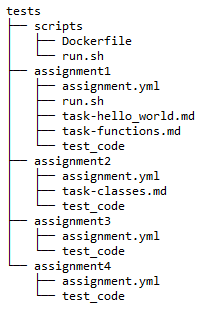
\includegraphics[scale=0.8]{photos/tests-repository-structure-tasks.PNG}
    \caption{Example of a tests repository with tasks}
    \label{fig:tests-repository-structure-tasks}
\end{figure}

As we see in the figure above, \textit{assignment1} and \textit{assignment2} both have tasks in them.

In essence we want these tasks to be represented as issues on all course group repositories.
This means that once a task is created by a teacher, and pushed to GitHub, the corresponding issues should be created on GitHub.
If a task is edited or deleted, QuickFeed must respectively either edit or delete the associated issue.
To manage the creation, deletion and editing of issues, QuickFeed's SCM API will be expanded to have such a capacity.

Beyond the ability to create, delete and edit issues, QuickFeed must be logically capable of determining when to perform these actions.
This means that QuickFeed will have to compare old tasks versus new ones, and then proceed accordingly.
We will therefore store representations of tasks in QuickFeed's internal database for this purpose.
Storing tasks also allows us to easily handle late enrolling groups, as we can use them to immediately create the required issues.

To edit issues, we will also need to internally store a reference to them in the database.

\subsection{Pull Requests}

The following questions are relevant for both this and the implementation part.

How do we listen to the webhook events that are relevant?
How do we single out the relevant events?
How should the pull requests be created?
How do we determine when to assign reviewers, when we do not have the ability to test based on tasks?
How do we ensure that reviewers are evenly distributed?
How do we ensure that reviewers are not assigned to their own repository?
What if a student pushes from a local branch that differs from a remote one?
What if an assignment is manually graded?

% To support pull requests, we need to expand

\subsection{Workflows}
